\section{Honeypot Fingerprinting Techniques}
\label{sec:hft}

%We now present various fingerprinting techniques for honeypots. The techniques are inferred from related work in the area of fingerprinting and contributions from researchers. Based on their type, we list four methods for fingerprinting of honeypots. Figure \ref{fig:taxonomy} summarizes the honeypot fingerprinting techniques. The taxonomy provides an overview of fingerprinting techniques and classifies them based on the approach. The techniques are further classified based on the detection and interaction models. The proposed taxonomy provides insights into efforts required for the determination of the honeypots. We classify the detection models .


Based on the background of fingerprinting research, we propose a taxonomy for honeypot fingerprinting. 
We propose a two tier taxonomy. The first tier classifies the fingerprinting techniques based on the detection methods.The second tier classifies the fingerprinting methods based on their interaction with the honeypots.
Tier 1 provides a top level outline of the honeypot fingerprinting techniques based on the detection scope. We principally classify them into Meta-data based, Probe based, Dependency based and Machine Learning Based techniques. Tier 2 further extends the classified techniques in Tier 1 to distinguish them into low and high effort techniques based on their interaction with the honeypots. This 2-Tier taxonomy provides an characteristic overview of the honeypot fingerprinting techniques. Figure \ref{fig:taxonomy} provides an overview of the Taxonomy based on Tier 1 and Tier 2. The rectangles represent Tier 1 and the squares represent Tier 2. We describe the tier based classifications in the below sub sections. 


\subsection{Meta-Data based fingerprinting}
Metadata based fingerprinting leverages the basic known information about the honeypot. This method is  not dependent on any interaction with the honeypot to determine any information. The technique utilizes basic information like the IP address or the domain name to infer the probability of honeypot existence. With IP address information, it is possible to determine other metadata about the system like the geo-location, ISP, AS, hosting or cloud provider. This metadata can be further analyzed to determine the probabilities of a honeypot. For example, if the target system has the TCP port 500 open and the IP address is geo-located to assigned to an University, it can be possible that the target system is a research honeypot. Another example would be if the same system is found to be hosted by a cloud provider like AWS, the system is likely a honeypot because Industrial Control Systems are physical devices that cannot be hosted or deployed on a cloud infrastructure.

Internet-wide scanning tools like Shodan provide honeypot detection services. Shodan uses active probing techniques and list the services active on the target systems. Shodan's  HoneyScore service accepts either an IP address or a URL to check in its database and provides feedback if the target system is a honeypot. Shodan describes that the service works by using the characteristics of known honeypots and assigning a score from 0.0 to 1.0 based on a match of the characteristics. The scores are stored in a native database. The service is still under development but is capable of detecting popular honeypots listed in Table \ref{tab:Table1}. Shodan also provides an API that can be used to integrate in scanning or fingerprinting scripts. The information collected by Shodan can be leveraged to determine the services running on the target system without interacting with the actual system. In addition, Shodan provides other essential metadata like HTTP content, response parameters, certificates and other technical parameters that can be used for fingerprinting. Other metadata-based fingerprinting methods include using search engines to collect information about the target system. Popular search engines crawl through the Internet daily to improve search results. With the search information, it is possible to identify and group relevant information to determine additional facts for the fingerprinting approach. 

\begin{figure}
    \centering
    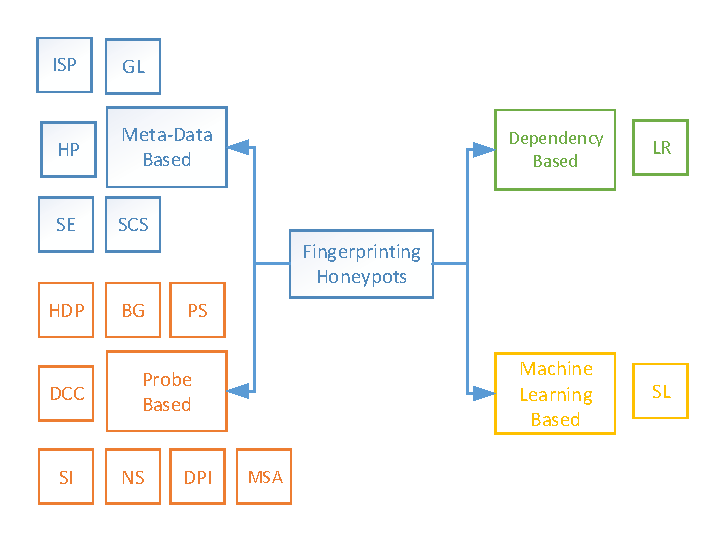
\includegraphics[scale=0.7]{taxonomy2}
    \caption{Honeypot Fingerprinting Taxonomy}
    \label{fig:taxonomy}
\end{figure}



Based on the information received from meta-data methods, it is possible to infer the existence of a honeypot with minimal interaction. We formulate the process of fingerprinting with the metadata approach based on the data received through the process. The parameters like geo-location provide information about the location of the honeypot. This information can be used to find relevance to the services rendered by the honeypot. For example, if the location is identified as an educational institution, the system is likely a honeypot deployed for experimental purposes. Similar inferences can be made with the data received from other parameters like ISP and hosting information. In the following subsections, we provide further information about the information that can be derived using metadata. 

\subsubsection{Geo-Location(GL)}
The location of a system determines what sector it is being used. It is possible to accurately determine the location of any system bearing a public IP address. This information is particularly useful when the system is suspected to be in a location that is not relevant to the services it is offering. This information can be used to derive that the target is either a training system or a honeypot. 

\subsubsection{\acrfull{isp}}
With the IP address information, it is possible to find the \acrshort{isp} that the address pool belongs to. This is especially useful in deriving information about the service providers to industries and corporate environments. Normally, enterprises have dedicated leased lines or fiber lines from well-known service providers. Also, service providers may deploy many honeypots in their management networks as a proactive defense strategy. For example, if the IP address is assigned to a hosting service like \acrshort{aws}, the \acrshort{isp} is listed as Amazon. This information can be used to infer that the system is a honeypot as Amazon is not a generic \acrshort{isp}. 

\subsubsection{Hosting Provider(HP)}
The hosting of the target system is good evidence of the implication of a honeypot. If the target is found to be hosted with a cloud provider, with pointless services, it is very conclusive that the target is a honeypot. Also, if the system is hosted with an unrelated domain pool that differs from the content of the honeypot, it can further lead to the inference of being a honeypot. It is very important for honeypot developers to create content and responses that relate to the hosting domain. 

\subsubsection{Social Engineering(SE)}
Social Engineering is a leading Offensive Security strategy. Most of the findings from other attackers are documented or reported on fingerprinting databases. Social engineering through Internet search engines can provide meta-data about honeypot signatures and fingerprinting information. Searching the metadata with sensible parameters on an advanced Internet search engine can provide interesting information about the target system. This information may include the past activity with the system, exploits, findings which can be used to infer that the target is a honeypot. The source of the information can be used in a scan script as a search database for fingerprinting. 

\subsubsection{Shodan/Censys Search (SCS)}
Shodan is a database of vulnerable systems on the Internet. It provides search as a service by accepting IP address, hostname or service names as search parameters. The output contains information about the target system and its open services. Shodan also provides a Honeypot Detection service called HoneyScore \cite{SHODAN} in addition to the database of vulnerable systems. Shodan performs daily scans of the Internet with probe-based fingerprinting methods to identify vulnerable systems on the Internet. It has also a major source for attackers to get fast access to vulnerable systems. Though Shodan and Censys use active probing to detect and collect technical information about the target systems, we leverage the information stored in their repositories as metadata to determine if the target system is a honeypot. Similarly, Censys provides advanced querying of the data collected from the internet wide scan. 

Censys is another Internet-wide search engine that is similar to Shodan. It makes use of the ZGRAB \cite{censys} utility to collect application-level data of the services running on the target machine. Censys also offers a query-able search based on the specific service running on the target system. Censys performs daily Internet-wide scans and aggregates the data in a query-able database. It differs from Shodan by providing a query-based search towards application-level data. Censys does not provide a honeypot detection service yet. Both Shodan and Censys provide reporting capabilities and offer API's. 

\subsection{Probe based fingerprinting}
\label{Probe Based}
Probe-based fingerprinting involves the creation of crafted queries to target devices to derive fingerprinting information. The probe-based methods engage with the target system, unlike the metadata methods. These methods focus on leveraging the responses from communication protocols and classifying the target machine based on specific values from the responses. Constructing probes is an advanced method that requires proficient knowledge of systems and protocols. Therefore extensive knowledge about systems and protocols is necessary for probe-based methods. The queries are constructed to trigger specific information from the target machine. The information may include system-specific unique values for parameters like initial congestion window (ICW) or re-transmission timeouts (RTO). 

Shu et al. \cite{shu2006network} proposed the fingerprinting of network protocols with a formal approach. The approach proposes a parameterized extended finite state machine (PEFSM) to formally model protocol specification and candidate conforming implementations. Several fingerprinting tools like NMap, Metasploit and Hydra make use probe-based methods to determine the operating systems and the protocol versions of the target systems. These tools rely on TCP packet information to determine the operating system. The specific values unique to each operating system are logged in the database of the tool. This helps in comparison to the value of parameters obtained by probing and determine the operating system by matching the closed parameter value from the database. We discuss different probe-based techniques in the following.

\subsubsection{Port Scanning(PS)}
Port scanning is the a technique to determine the open ports and services on the target system. It forms the first step before attacking a target system. Port scanning involves scanning and listing open ports on the target system. Ports that are open signify that they are open for communication and the active services on the system. Many administrators leave the services running on default ports and configuration. For example, port 22 is used for SSH and port 80 for HTTP web service. Port scanning provides information about the transport layer protocol used, the port number and the status of the port. Popular port scanning tools like NMap\cite{NMap} provide more information about the open ports like the active service, version and the vulnerabilities associated with the version. NMap also provides fast scans and detailed scans that recognizes six port states and classifies them into open, closed, filtered, unfiltered, open-filtered and closed-filtered. It has a database of fingerprinting information for 2000 services. 
Tools like NMap and ZMap \cite{zmap} provide parameterized scripts to run port scanning on target machines. Furthermore, custom scripts have been developed with NMap that can identify honeypots like Kippo and Dionaea.  

\subsubsection{Banner Grabbing(BG)}
Banner grabbing is one of the techniques used in the reconnaissance process following a port scan. After learning about the open ports, a connection is established with the remote system to get information about the service and the version number. Some implementations of protocols like FTP and HTTP expose critical system information like service name, software, version, and the operating system. Banner grabbing based probes targeted on a protocol can reveal vulnerabilities associated with any critical information obtained. The CVE database \cite{CVE} provides a list of vulnerabilities associated with protocols, software and operating systems. Popular tools for Banner Grabbing are Wget\cite{wget}, cURL\cite{curl}, NMap\cite{NMap}, Netcat\cite{netcat}, and Dmitry\cite{dmitry}. Banner grabbing can be used not only for netfork fingerprinting, but also for application fingerprinting. Damron et. al \cite{bannergrab} demonstrates that banner grabbing can be effectively used to fingerprint application software through requests. The author considers Apache Web Server as an example and presents distinct response codes from the banner that can be used fingerprinting. Alexander et. al \cite{Vetterl2018} show that banner response from honeypots like Kippo showcase distinct values that can be used for fingerprinting the honeypot. Censys also provides a feature for querying the database with specific values in the banner response. Banner grabbing is also an integrated feature with port scanning on most of the port scanning tools. 

\subsubsection{Handshake Proposals(HSP)}
TLS handshake is a protocol process that establishes the parameters for secure communication between systems. The handshake process involves the exchange of messages to acknowledge each other, the TLS version,  negotiate the cipher suites, authentication with the public key and session keys generation. Besides, there are parameters like message size and timestamp. TLS negotiations are transmitted in plaintext. With the information available through this negotiation, it is possible to fingerprint the client and server applications.  The handshakes also determine the cipher suites proposed by the target system. This information can be leveraged to find vulnerabilities and to characterize the systems based on limited choice of ciphers. The handshake process provides information about the server system that can be used for fingerprinting. As many honeypots depend on static libraries, careful comparison of the actual and the target system responses can reveal if the target system is a honeypot. 
JA3 and JA3s\cite{JA3} are techniques developed that can actively fingerprint the TLS client and servers based on their hello messages. 



\subsubsection{\acrfull{dpi}}
\acrfull{dpi}  is a method for analyzing and monitoring network traffic. Using DPI, network packets can be filtered based on the protocol type and the data in packet components. Conventional packet inspection methods examine only the header information for filtering the traffic. DPI is performed at enterprises using layer 6 devices like firewalls or intrusion detection systems. DPI can help to identify redundant responses received from a machine for fingerprinting purposes. DPI relies on a repository of existing protocol fingerprints for classification. It is an effective technique used by IDS to filter malicious packets from the production networks. On the contrary, DPI can be an effective technique to fingerprint honeypots or protocols based on the header and the payload information. Sang et al.\cite{Sang} proposed a fingerprinting technique based on byte embedding for the classification of network protocols. The approach learns the application fingerprints from traffic traces by characterizing the packet payloads with a byte embedding based payload alignment algorithm. However, with open-source libraries and tools like nDPI\cite{nDPI}, it is possible to fingerprint and inspect various protocol services on the honeypot. DPI requires good knowledge of packet-level communication and networking. It is an advanced probe-based method that requires advanced knowledge for the creation of probes to retrieve specific information from the target system.  


\begin{table}
\begin{tabular}{||c c c c c||} 
 \hline
 Honeypot & Protocol & Language & Library & Updated \\ [0.5ex] 
 \hline
 Kippo  & SSH    & Python &  TwistedConch & May2015 \\ 
 Cowrie & SSH    & Python &  TwistedConch & May2018 \\
 TPwD   & Telnet & C      &  custom       & Feb2016 \\
 MTPoT  & Telnet & Python &  telnetsrv    & Mar2017 \\
 TIoT   & Telnet & Python &  custom       & May2017 \\
 Cowrie & Telnet & Python &  TwistedConch & May2018 \\
 Dionaea& HTTP   & Python &  custom       & Sep2016 \\
 Glastof& HTTP   & Python &  BaseHTTPServer& Oct2016 \\
 Conpot & HTTP   & Python &  BaseHTTPServer& Mar2018 \\ [1ex] 
 \hline
\end{tabular}
\caption{Library references in honeypots}
\label{library}
\end{table}



\subsubsection{Default Configuration Check(DCC)}
Applications are setup with setup scripts or by using install media. Often, these media do not prompt the user to change the default settings or configuration before the final installation. This leaves the system running with a default configuration. For example, we have Apache Tomcat Manager instance running on a default installation of Apache Tomcat. The manager provides an interface to manage the web service and the deployments. It is important to configure the tomcat manager or disable if not used. Similarly, devices and applications are running with default configurations on the Internet. With these default configurations, it is easily possible to fingerprint the target system. Honeypots like Kippo, Cowrie, Glastopf, and Conpot are usually deployed with default configurations. Morishita et al. \cite{morishita} provides an approach to self-revealing honeypots on the Internet by detection through default configurations.  This leads to the easy discovery of honeypots by constructing a probe to check the default configuration. If the response matches the defaults, the end systems is likely a honeypot.
\newline
\subsubsection{System information(SI)}
Systems often reveal or allow to be queried about specific information like the processor family, architecture, network interface and timezone. This specific information help in the inference of a honeypot system. They are useful metadata when combined with data collected from other techniques.  Also, ping response times can be used to detect the operating system of the target system. Early works from Mukkamala et al. \cite{mukkamala} show the detection of low-interaction honeypots and virtual environments based on support vector machine models. The approach compares the average time taken for responses from a virtual machine than that of a real system. The authors determine the existence of a honeypot by testing the limitations of the services emulated by the honeypot, timing analysis of the ICMP echo requests and TCP/IP fingerprinting with 49 featured data set.  
\newline
\subsubsection{Network Sniffing(NS)}
Network Sniffing is a reconnaissance method used for analyzing the network traffic exchanged between two entities. The traffic is monitored to find anomalies. Any deviation from regular behavior, such as redundant network traffic, broadcasts and logging are easy signs of a honeypot . Sniffing techniques work well if the packet sniffing tools are installed within the same network as a honeypot\evc{I don't get these 2 sentences}. These techniques are also effective to determine the existence of high-interaction honeypots\evc{how?}. However, sniffing methods are ineffective if the attacker is unable to filter packets from the source system. Attackers can still use sniffing techniques if they gain successful access to a vulnerable system. The attackers can install bots to tap the network traffic and have them report to a C\&C \evc{abbreviation?} server. This can expose other systems in the network of the honeypot. \evc{paragraph not very clear}

\subsubsection{Multi-stage attacks(MSA)}
Multi-stage attacks can be defined as a sequential array of exploits by an attacker targeting multiple vulnerable services on a system. Multi-stage attacks leverage the vulnerable service on the system to exploit the other services on the same system by gaining more control over the system. These kinds of attacks are key to detection as they help in inferring a relationship between multiple services running on the system that constitutes an environment. Vasilomanolakis et al. \cite{vasilomanolakis} proposed a honeypot capable of identifying multi-stage attacks. The honeypot is capable of simulating environments by running related services. The honeypot effectively captures advanced persistent threats. However, the information about services running on a system can also infer that the system is not real. For example, in the case of \acrshort{ics}, the communication protocols are active on specific devices and not on a single device. Honeypots like Conpot that are based on \acrshort{ics} show that all the services are running on the target machine. Hence, it can be easily inferred that the target system is a honeypot. 

% will be added in countermeasures 
%\subsubsection{Risks in Probe-Based Fingerprinting}
%\evc{how is this paragraph relevant compared to the previous ones?}
%However, there are risks involved in probe-based fingerprinting methods. As these methods involve direct interaction with the target system, eventually the probe system is blacklisted. We must remember that there is no real reason for establishing a connection with a honeypot. Any connections observed with a honeypot is considered potentially an attack. Probing systems may get blocked by this approach. This limits in further exploitation or identification of the attacker or the honeypot. It is important to keep the attacker engaged with the honeypot to collect as much possible to identify the attacker. 

\subsection{Dependency-based fingerprinting}
Honeypots simulate network protocols. The simulations are usually implemented using pre-built language-specific libraries of protocols that are open-source \cite{Vetterl2018}. Many of the referenced libraries are very old and not maintained. Developers often reference libraries in their project to save time building the library themselves. These libraries are not developed to fully emulate network protocols. They offer basic communication features with some hardcoded response strings. Popular open-source honeypots binaries are available on the Internet. By carefully observing the source code, or the referenced libraries, it is possible to create probes that trigger the static response from the referenced library. For example, the Twisted Conch \cite{twisted}  library is the most referenced library for SSH protocol simulations in honeypot implementations \cite{counting}. Though there have been recent contributions to the library, there is no change or update made on the honeypots referencing it. Since the library is available as open-source, it can be analyzed for its simulations and static responses can be detected for specially developed probes. The Twisted Conch library also includes simulation for the Telnet protocol. Dependency based detection is an effective method for detecting honeypots based on SSH, HTTP, Telnet, FTP, and Modbus protocols because of their dependency to static libraries. Many honeypots refer to static libraries and this causes static response for carefully crafted requests.There are limited libraries available for the simulation of the above protocols. The honeypots are not updated and still use static responses emulated by the libraries. Table \ref{library} \cite{Vetterl2018} shows the list of libraries referenced by popular honeypots, protocols, and their versions. 



\subsection{\acrfull{ml} based fingerprinting}
\acrfull{ml} techniques are based on the response data received from probe-based methods. The collection of response data acts as a learning dataset for designing a model for the detection of honeypots. The \acrshort{ml} models depend on data and modeling algorithms to learn the process of fingerprinting based on previous inference in the data set. Huang et al.  provide an \acrshort{ml}-based model approach to detect honeypots\cite{huang}. The approach introduces features from the network layer, application layer, and the operating system layer and proposes a detection model to identify honeypots with a stated detection rate of 0.03 AUC. Feng et al. \cite{Feng2016} also propose a learning model based on the probe-based method for detecting \acrshort{ics} honeypots. The proposed method initially uses reconnaissance to identify systems open to the Internet with specific ports open which are related to \acrshort{ics}. Next, they construct probes to collect data for specific banners and handshakes. This information is used to design a learning model to classify real systems and honeypots of \acrshort{ics} devices.

\acrshort{ml}-based fingerprinting is recommended when there is enough data to train the supervised learning process. With good learning models and data, it is possible to increase the detection accuracy. This technique is suitable to be applied after successful fingerprinting methods are established for a honeypot through metadata and probe-based fingerprinting techniques. Supervised learning relies on good training data set for its classification. The training data set must be relevant for incorporating new features. The main drawback of this approach is the freshness of the data. The data on which the models are based need to be constantly changed and tested to ensure that the detection accuracy is still maintained. Unsupervised learning techniques can be applicable in such situations. 
